%% polematrix documentation
%% Copyright (C) 2017 Jan Felix Schmidt <janschmidt@mailbox.org>
%%   
%% This program is free software: you can redistribute it and/or modify
%% it under the terms of the GNU General Public License as published by
%% the Free Software Foundation, either version 3 of the License, or
%% (at your option) any later version.
%%
%% This program is distributed in the hope that it will be useful,
%% but WITHOUT ANY WARRANTY; without even the implied warranty of
%% MERCHANTABILITY or FITNESS FOR A PARTICULAR PURPOSE.  See the
%% GNU General Public License for more details.
%%
%% You should have received a copy of the GNU General Public License
%% along with this program.  If not, see <http://www.gnu.org/licenses/>.

\documentclass[a4paper]{scrartcl}
\usepackage[english]{babel}
\usepackage[utf8]{inputenc}
\usepackage[T1]{fontenc}
\usepackage[margin=2.5cm]{geometry}
\usepackage{siunitx}
\usepackage{csquotes}
\usepackage{booktabs}
\usepackage{multicol}
\usepackage{amsmath}
\usepackage[colorlinks,linkcolor=blue,citecolor=magenta,urlcolor=teal]{hyperref}
\usepackage[backend=biber,style=alphabetic,backref]{biblatex}
\usepackage{todonotes}

\usepackage{polem_defs}
\usepackage{cleveref}

\author{Jan Felix Schmidt \textless janschmidt@mailbox.org\textgreater}
\title{polematrix}
\subtitle{a spin tracking code for electron accelerators using elegant}
\date{documentation for version 0.99}

\hypersetup{
  pdftitle={polematrix documentation},
  pdfauthor={Jan Felix Schmidt}
}

\bibliography{polem}

\setcounter{tocdepth}{2}

\begin{document}
\maketitle

\begin{abstract}
  \polem is a spin tracking code. It calculates the motion of the spin of ultra
  relativistic electrons in particle accelerators. It implements a simple matrix tracking
  as multi-thread \cpp application. The input can be any lattice file from \ele or
  \madx. All required particle trajectories are also imported from the established
  particle tracking codes \ele or \madx.

  \polem includes synchrotron radiation via import from \ele or an own implementation of
  longitudinal phasespace. A short description of \polem is given in the IPAC'16
  contribution \cite{IPAC16-decoh} and in my phd thesis, which will be available soon (in
  German).
  
  Do not hesitate to contact me if you have any questions and please report bugs.
\end{abstract}

\tableofcontents
\clearpage


\section{\polem can}
\label{sec:polem-can}
\todo[inline]{list}

\section{\polem cannot}
\label{sec:polem-cannot}
\todo[inline]{list}


\section{Coordinate System}
\label{sec:coord}

\begin{figure}
  \centering
  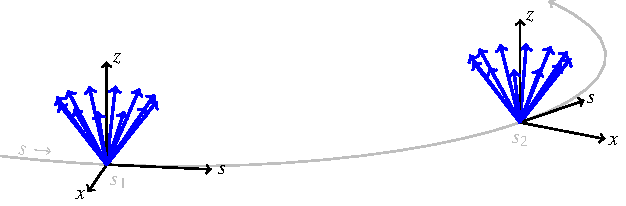
\includegraphics{coord}
  \caption{Accelerator coordinate system and precessing spin vectors. \cite{dr}}
  \label{fig:coord}
\end{figure}

% Coordinate System
\polem uses the typical accelerator coordinate system sketched in \cref{fig:coord}, which
is moving along the reference orbit. The position along the reference orbit is called $s$.
Since \polem assumes ultra relativistic electrons, the velocity along $s$ is assumed to be
constant $v\approx c$ and the position is alternatively parametrized by the time
$t = s/c$, which increases linearly for multiple turns in a circular accelerator. $t$ is
used to define the duration and output step width of the spin tracking.

At each position $s$ the $x$ axis points in horizontal direction and the $z$ axis points
in vertical direction. $z>0$ is above the reference orbit. In a circular electron
accelerator $x>0$ corresponds to the outer side of the ring (to larger radii of the
bending magnets). The longitudinal axis is also referred to as $s$ axis.

% Spin and Polarization Vectors
Accordingly, the tracked spin vectors $\svec[i](t)$ are parametrized as horizontal
component \sx, vertical component \sz and longitudinal component \slong. The same
coordinate system is used for the resulting polarization vector $\pvec(t)$.







\section{Usage}
\label{sec:usage}

\subsection{Execution}
\label{sec:execution}

\polem is called via
\begin{bashcode}
  polematrix [options] [CONFIGURATION FILE]
\end{bashcode}
where \bashinline{[options]} are the command line options shown in
\cref{tab:polem-options}. All parameters of the spin tracking can be set up in an \xml
configuration file (\bashinline{[CONFIGURATION FILE]}) which is described in
\cref{sec:config}.
%
The lattice of the accelerator is given as any conventional \ele or \madx lattice file and
is set in the configuration file (see \cref{sec:config}). A template configuration file
with default values can be generated anytime by executing \bashinline{polematrix --template}.


\begin{table}[h]
  \centering
  \begin{tabular}{ll}
    \toprule
    \bashinline{-h [ --help ]}              &  display this help message \\
    \bashinline{-V [ --version ]}           &  display version \\
    \bashinline{-T [ --template ]}          &  create config file template (\bashinline{template.pole}) and quit \\
    \bashinline{-R [ --resonance-strengths ]} &  estimate resonance strengths instead of spin tracking \\
    \midrule
    \bashinline{-t [ --threads ] arg (=all)}     &  set number of threads used for tracking \\
    \bashinline{-o [ --output-path ] arg (=.)}   &  path for output files \\
    \bashinline{-v [ --verbose ]}            &  activate additional status output \\
    \bashinline{-n [ --no-progressbar ]}     &  do not show progress bar during tracking\\
                                            &  (e.g. if output is redirected to a log file)\\
    \bashinline{-a [ --all ]}                &  write additional output files (e.g. lattice und orbit) \\
    \bashinline{-s [ --spintune ] arg}       &  in resonance strengths mode (\bashinline{-R}):\\
                                            &  calculate for given spin tune only\\
    \bottomrule
  \end{tabular}
  \caption{Command line options of \polem.}
  \label{tab:polem-options}
\end{table}

\subsection{Output}
\label{sec:output}

The components of each spin vector $\svec[i](t)$ is written to the text file
\bashinline{spins/spin_i.dat} in the output path during tracking. The output step width
can be set in the configuration file (see \cref{sec:config-spintrk}). When tracking is
completed for all spins, the polarization vector $\pvec(t)$ is calculated for each output
step as average over all successfully tracked spins. It is saved as
\bashinline{polarization.dat} in the output path.


\section{Installation}
\label{sec:installation}

\polem has been tested only on Ubuntu/Debian Linux with the GCC compiler so far.

\subsection{Dependencies}
\label{sec:dependencies}

\polem requires the following programs and libraries:
\begin{multicols}{2}
\begin{itemize}
\item GCC compiler
\item CMake
\item Gnu Scientific Library (GSL) \cite{gsl}
\item Boost program options
\item Boost filesystem
\item Boost property tree %\cite{boost-pt}
\item Boost random %\cite{boost-random}
\item Armadillo library \cite{arma}
\item \pal library \cite{palattice}
\end{itemize}
\end{multicols}
\pal is available on github. The source code can be downloaded at \cite{palattice} and
compiled and installed as described in the enclosed README file.
%
All other dependencies may be in the package repositories of your Linux distribution. On
Ubuntu you can install all required packages with the following command:
\begin{bashcode}
  sudo apt-get install g++ cmake libgsl-dev libboost-dev libboost-program-options-dev libboost-filesystem-dev libarmadillo-dev
\end{bashcode}
Additionally, \polem relies on the established particle
tracking program \ele (or \madx), whose lattice files and tracking results are used for
spin tracking.  \ele (and \madx) can be configured and execute automatically by \polem using
\pal. The installation of \ele and \madx is described in \cref{sec:elemadx}.


    
\subsection{Build and Install \polem}
\label{sec:build}
\polem is compiled and installed using \software{CMake} with the following commands:
\begin{bashcode}
  cd polematrix/build
  cmake ../
  make
  sudo make install
\end{bashcode}
The default install path is \bashinline{/usr/local/bin}. It can be changed by setting the
\bashinline{CMAKE_INSTALL_PREFIX} variable in \bashinline{polematrix/CMakeLists.txt}.
%
To uninstall \polem run
\begin{bashcode}
  cd polematrix/build
  sudo make uninstall
\end{bashcode}



\subsection{Underlying Particle Tracking Programs}
\label{sec:elemadx}

I recommend to use \polem with \ele since much more tracking parameters can be set
automatically -- including number of particles (starting with a Gaussian profile in
radiation equilibrium), tracking duration and linear energy ramps. If you have only a
lattice file in \madx format, you can convert it automatically to an \ele lattice
using the program \software{convertlattice} which is included in \pal \cite{palattice}.

\subsubsection{\ele}
\label{sec:ele}
The particle tracking program \ele \cite{elegant} is developed at the Advanced Photon
Source at Argonne National Laboratory. Packages for many operating systems can be
downloaded at \cite{elegant-download}. Also install the \software{SDDSToolKit}, which is
needed to access the binary output files of \ele.
%
If there is no package for your system, you can download the \bashinline{Build-AOP-RPMs}
script instead which automatically builds all desired programs from source (see the guide
in \cref{sec:ele-install}).
%
There is a parallel version of \ele, called \software{Pelegant}, which speeds up the
tracking \cite{pelegant} (installation hints in \cref{sec:ele-install}). The \ele manual
can be found at \cite{elegant-manual}.

\subsubsection{\madx}
\label{sec:madx}
The particle tracking program \madx is developed at CERN and can be downloaded from the
website \cite{madx}, which also provides the \madx manual.






\section{Configuration File Reference}
\label{sec:config}

\polem is configured with an \xml file. The individual entries are arranged in several
thematic groups like this:
\begin{xmlcode}
  <groupA>
    <entry1> value </entry1>
    <entry2> value </entry2>
  </groupA>
  <groupB>
    <entry42> value </entry42>
  </groupB>
\end{xmlcode}
The order of groups and entries is arbitrary. Many entries have default values and must
not be set. When \polem is executed, a configuration file with the actual values of all
entries is saved as \bashinline{currentconfig.pole}. All entries are
documented in the following.

\subsection{spintracking}
\label{sec:config-spintrk}

The group \xmlinline{<spintracking>} contains the setup of the spin tracking itself.\\[2mm]

\begin{configdoc}{t_start}{double}{\si{\s}}[0.0]
  The start time $t_\text{start}$ of the spin tracking
\end{configdoc}

\begin{configdoc}{t_stop}{double}{\si{\s}}
  The stop time $t_\text{stop}$ of the spin tracking
\end{configdoc}

\begin{configdoc}{E0}{double}{\si{\GeV}}
  Beam energy at the time $t=\SI{0}{\s}$
\end{configdoc}

\begin{configdoc}{dE}{double}{\si{\GeV\per\s}}
  Speed of the linear energy ramp
\end{configdoc}

\begin{configdoc}{Emax}{double}{\si{\GeV}}[\num{e10}]
  Maximum energy to confine the energy ramp.
  If the energy ramp reaches this energy, it is kept until the end of the tracking. Use a
  sufficiently large number do disable this feature (default).
\end{configdoc}

\begin{configdocgroup}{s_start}
  Initial value of the spin vector $\svec(t_\text{start})$. It is used for all spins.
  Thus, the tracking always starts with polarization $\pabs(t_\text{start}) = 1$. The
  three components of the vector are each set as a separate entry:
  
  \begin{configdoc}{x}{double}{}[0.0]
    Horizontal component \sx of the initial value
  \end{configdoc}

  \begin{configdoc}{z}{double}{}[1.0]
    Vertical component \sz of the initial value
  \end{configdoc}

  \begin{configdoc}{s}{double}{}[0.0]
    Longitudinal component \slong of the initial value
  \end{configdoc}
\end{configdocgroup}

\begin{configdoc}{numParticles}{unsigned int}{}[1]
  Number of particles (spin vectors) for the spin tracking
\end{configdoc}

\begin{configdoc}{dt_out}{double}{\si{\s}}[$(t_\text{stop}-t_\text{start})/1000$]
  Step width of the output of \pvec and \svec[i]
\end{configdoc}

\begin{configdoc}{gammaModel}{string}{}[radiation]
  Model for longitudinal beam dynamics $\gamma_i(t)$ during spin tracking. The two
  realistic and three simple models are discussed in \cite[chapter~4]{dr}.
  \begin{description}
  \item[\xmlinline{radiation}] This model is implemented in \polem and calculates
    stochastic emission of synchrotron radiation.
  \item[\xmlinline{simtool}] $\gamma_i(t)$ is imported from the particle tracking program,
    which is selected as \xmlinline{<simTool>} in the group \xmlinline{<palattice>} (see below).
    I recommend to use this model with \ele.
  \item[\xmlinline{linear}] Deactivation of longitudinal dynamics. All particles just
    follow the linear energy ramp: $\gamma_i(t) = \gcentral$.
  \item[\xmlinline{offset}] Every particle gets an energy offset, which is constant over
    time: $\gamma_i(t) = \gcentral + \Delta\gamma_i$.
  \item[\xmlinline{oscillation}] Approximation of longitudinal dynamics by harmonic
    oscillations:\\$\gamma_i(t) = \gcentral + \Delta\gamma_i \cos(\ws t + \psi_i)$
  \end{description}
\end{configdoc}

\begin{configdoc}{trajectoryModel}{string}{}[closed orbit]
  Model for transverse particle trajectories $x_i(t)$ and
  $z_i(t)$ during spin tracking. To date, two models are available:
  \begin{description}
  \item[\xmlinline{closed orbit}] The closed orbit is used as trajectory for all
    particles. Thereby, all spins experience the same magnetic fields, which exclusively
    consist of revolution harmonic contributions (apart from explicitly time dependent
    fields). The closed orbit can be determined without particle tracking. This model is
    sufficient if the simulation of intrinsic resonances is not necessary.
  \item[\xmlinline{trajectory}] The individual trajectories are imported from the particle
    tracking program selected as \xmlinline{<simTool>} in the group
    \xmlinline{<palattice>} below. The particle tracking is executed automatically.
  \end{description}
\end{configdoc}

\begin{configdoc}{edgeFocussing}{bool}{}[false]
  Switch to enable horizontal magnetic fields at the edges of dipole magnets (edge
  focusing) during the spin tracking. Can be activated with \xmlinline{true} or
  \xmlinline{1} and deactivated with \xmlinline{false} or \xmlinline{0}.
\end{configdoc}




\subsection{palattice}
\label{sec:config-pal}
The group \xmlinline{<palattice>} contains the configuration of lattice import and
particle tracking.\\[2mm]

\begin{configdoc}{simTool}{string}{}
  Selection of the simulation tool for lattice import and particle tracking. Possible values:
  \xmlinline{elegant} or \xmlinline{madx}. I recommend using \ele since much more tracking
  parameters can be set automatically -- including number of particles, tracking duration
  and linear energy ramps. A \madx lattice can be converted automatically to an \ele
  lattice using \pal.
\end{configdoc}

\begin{configdoc}{mode}{string}{}
  Selection of import mode:
  \begin{description}
  \item[\xmlinline{online}] The simulation tool is configured and executed automatically.
    Typically, this mode should be used.
  \item[\xmlinline{offline}] In this mode the simulation tool is not executed. Instead,
    existing output files are imported. This can be helpful to avoid repeated execution of
    a particle tracking or to use \polem if \ele and \madx are not available.
  \end{description}
\end{configdoc}

\begin{configdoc}{file}{string}{}
  Lattice file for spin tracking. The file format has to be suitable for the program
  selected as \xmlinline{<simTool>}.
  Depending on \xmlinline{<mode>} varying files must be given:
  \begin{itemize}
  \item In \xmlinline{online} mode \xmlinline{<file>} is the lattice file
    (\bashinline{.lte} for \ele, usually \bashinline{.madx} for \madx).
  \item In \xmlinline{offline} mode \xmlinline{<file>} is the \bashinline{.param} output
    file (\ele) and the \bashinline{.twiss} output file (\madx) respectively.
  \end{itemize}
\end{configdoc}


\begin{configdoc}{saveGamma}{string}{}[]
  This option is meaningful only with \xmlinline{<gammaModel>} \xmlinline{simtool}. It
  allows to export the $\gamma_i(t)$, which are imported from the particle tracking, to
  text files. The option contains a list of particle numbers $i$ for the export.
  %
  The particle numbers are delimited by commas (e.g. \xmlinline{0,2,7}). Additionally,
  ranges of numbers can be given by hyphens (e.g. \xmlinline{0,3-6,8}). The text files are
  saved as \bashinline{gammaSimTool_i.dat} (particle number $i$).

  \textbf{Attention:} The \ele \bashinline{particleIDs} start at 1. This particle is
  assigned to particle number 0 in \polem.
\end{configdoc}

\begin{configdocgroup}{simToolRamp}
  If an \ele tracking is executed, the energy ramp configured in the group
  \xmlinline{<spintracking>} can be set for the particle tracking automatically. This is
  not implemented for \madx.

  \begin{configdoc}{set}{bool}{}[true]
    Switch for the energy ramp transfer to \ele. Can be activated with \xmlinline{true} or
    \xmlinline{1} and deactivated with \xmlinline{false} or \xmlinline{0}.
  \end{configdoc}

  \begin{configdoc}{steps}{unsigned int}{}[200]
    If the transfer is active, the ramp is calculated at discrete sampling points, which
    are then written to a \sdds file. Here, the number of sampling points can be changed.
    They are distributed equidistant from $t_\text{start}$ to $t_\text{stop}$.
  \end{configdoc}
\end{configdocgroup}

\begin{configdocgroup}{rfMagnets}
  These options can be used to configure the magnetic field $B$ of any lattice element as a
  time dependent alternating field (rf field)
  \begin{equation*}
    B(T) = B \cdot \cos\left( 2\pi \left[ Q_\text{rf,1}T + \frac{1}{2}\Delta
        Q_\text{rf} T^2 \right] \right)
  \end{equation*}
  as a function of the turn $T$.
  The setup only affects the spin tracking and not the particle tracking with \ele or
  \madx. In addition, the field has to be set up in \ele/\madx, if the influence of an rf
  field on beam dynamics should be included.

  An arbitrary number of elements can be set up with an rf field since all
  following options allow for giving multiple values as a comma separated list. All
  options must have the same number of entries, which are then assigned to the
  corresponding elements in \xmlinline{<elements>}.\\[1mm]

  \begin{configdoc}{elements}{string}{}[]
    Name of the element for rf field. [multiple elements as comma separated list]
  \end{configdoc}

  \begin{configdoc}{Q1}{string}{}[]
    Frequency of the rf field at the beginning of the spin tracking (turn $T=1$) normalized to
    the revolution frequency (tune $Q_\text{rf,1}$). [for multiple elements as comma separated list]
  \end{configdoc}

  \begin{configdoc}{dQ}{string}{}[]
    Frequency change per turn (frequency sweep) -- also as a tune $\Delta Q_\text{rf}$.
    [for multiple elements as comma separated list]
  \end{configdoc}

  \begin{configdoc}{period}{string}{}[]
    Duration of the frequency sweep in turns. After this period the sweep starts again.
    [for multiple elements as comma separated list]
  \end{configdoc}
\end{configdocgroup}



\subsection{radiation}
\label{sec:config-rad}
This group is for configuration of the \xmlinline{<gammaModel>} \xmlinline{radiation},
which is a model of longitudinal dynamics implemented in \polem to allow for a stochastic
synchrotron radiation model without import from a particle tracking program. If another
\xmlinline{<gammaModel>} is selected, the whole group can be ignored.


\begin{configdoc}{seed}{int}{}[\textit{random}]
  The seed of the random number generator, which is used for the initial particle
  distribution in phase space and the stochastic photon emission.
\end{configdoc}

\begin{configdocgroup}{savePhaseSpace}
  Here, particle numbers $i$ can be chosen for a plain text export of longitudinal phase
  space $(\phf,\gamma)$ -- analog to \xmlinline{<saveGamma>} in group
  \xmlinline{<palattice>}.

  \begin{configdoc}{list}{string}{}[]
    A list of particle numbers $i$ for the export. The particle numbers are delimited by
    commas (e.g. \xmlinline{0,2,7}). Additionally, ranges of numbers can be given by
    hyphens (e.g. \xmlinline{0,3-6,8}). The text files are saved as
    \bashinline{longPhaseSpace_i.dat} (particle number $i$).
  \end{configdoc}

  \begin{configdoc}{elementName}{string}{}[]
    The name of an element in the lattice. The phase space coordinates are recorded at the
    position of this element. This option must be set to use \xmlinline{<savePhaseSpace>}.
    Else no output is written.
  \end{configdoc}
\end{configdocgroup}

\begin{configdocgroup}{startDistribution}
  \polem calculates the initial phase space coordinates of all particles so that the
  $\phf_i$ and the $\gamma_i$ are Gaussian distributed and average and width of the
  distribution correspond to the radiation equilibrium. The following two options can be
  used to vary the width  of these distributions.

  \begin{configdoc}{sigmaPhaseFactor}{double}{}[1.0]
    Factor to scale the width of the Gaussian distribution of the phases $\phf_i$. A value
    of 1 corresponds to the radiation equilibrium.
  \end{configdoc}

  \begin{configdoc}{sigmaGammaFactor}{double}{}[1.0]
    Factor to scale the width of the Gaussian distribution of the particle energies
    $\gamma_i$. A value of 1 corresponds to the radiation equilibrium.
  \end{configdoc}
\end{configdocgroup}


The following options are physics parameters of the accelerator, which are required by the
synchrotron radiation model. They are determined by the particle tracking program and
imported automatically if the corresponding option is not set here (default value
\num{0.0}). Thus, these options can be used to enforce other values.\\[2mm]

\begin{configdoc}{momentum_compaction_factor}{double}{}[0.0]
  the momentum compaction factor \alphac
\end{configdoc}

\begin{configdoc}{momentum_compaction_factor_2}{double}{}[0.0]
   the second order momentum compaction factor \alphactwo
\end{configdoc}

\begin{configdoc}{overvoltage_factor}{double}{}[0.0]
  the overvoltage factor $q$
\end{configdoc}

\begin{configdoc}{harmonic_number}{unsigned int}{}[0]
  the harmonic number $h$
\end{configdoc}

\begin{configdoc}{bending_radius}{double}{\si{\m}}[0.0]
  the average bending radius $R$ of the dipole magnets
\end{configdoc}

\begin{configdoc}{longitudinal_damping_partition_number}{double}{}[0.0]
  the longitudinal damping partition number $J_s$
\end{configdoc}



\subsection{resonancestrengths}
\label{sec:config-resstr}
This group is for configuration of the estimation of resonance strengths of depolarizing
resonances. This special mode can be activated by the command line option \bashinline{-R}.
If \polem is used for spin tracking, the whole group can be omitted.\\[2mm]

\begin{configdocgroup}{spintune}
  The resonance strength is calculated for discrete values of the spin tune \ga and
  written to the text file \bashinline{resonance-strengths.dat}. Here, the output range and
  step width can be set.

  \begin{configdoc}{min}{double}{}[0.0]
    minimum spin tune \ga
  \end{configdoc}

  \begin{configdoc}{max}{double}{}[10.0]
    maximum spin tune \ga
  \end{configdoc}

  \begin{configdoc}{step}{double}{}[1.0]
    step width $\Delta\ga$ for calculation and output of the spin tune
  \end{configdoc}
\end{configdocgroup}

\begin{configdoc}{turns}{unsigned int}{}[0]
  If the resonance strengths are calculated for non integer \ga, multiple particles with
  their individual trajectories have to be taken into account and the resulting resonance
  strength is the average over all particles. For this purpose, the trajectories are
  imported from the particle tracking program as it is configured in the group
  \xmlinline{<palattice>}. The number of particles is taken from the option
  \xmlinline{<numParticles>} (Gruppe \xmlinline{<spintracking>}).

  Here the number of turns $N_u$ for the trajectories can bes set. If the default value 0
  is used, the number of turns is set automatically according to the minimum number
  required for the chosen frequency resolution \xmlinline{<step>}: $N_u = 1/\Delta\ga$.
\end{configdoc}



\clearpage
\appendix

\section{\ele Installation Guide}
\label{sec:ele-install}

\todo[inline]{guide}


\printbibliography[heading=bibintoc]

\end{document}



%%% Local Variables: 
%%% mode: Latex
%%% LaTeX-command: "latex -shell-escape"
%%% End: 
